\documentclass[a4paper]{article}
\usepackage[a4paper,margin=0mm]{geometry}
\usepackage{fontspec}
\usepackage{unicode-math}
\usepackage{tikz}
\usetikzlibrary{calc}
\usepackage[table]{xcolor}
\usepackage[absolute]{textpos}
\usepackage{enumitem}
\usepackage{array}
\usepackage{multirow}

\setmainfont{Libertinus Serif}
\setsansfont{Libertinus Sans}
\setmathfont{Libertinus Math}

\definecolor{accent}{HTML}{0F6A52}
\definecolor{badge}{HTML}{A9CFC2}
\definecolor{ink}{HTML}{2A2E30}

\setlength{\TPHorizModule}{1mm}
\setlength{\TPVertModule}{1mm}
\setlength{\parindent}{0pt}
\pagestyle{empty}
\binoppenalty=10000 \relpenalty=10000

\newcommand{\LCOL}{16mm}
\newcommand{\RCOL}{111mm}
\newcommand{\COLW}{83mm}

\newcommand{\topicheader}[2]{%
\begin{textblock*}{194mm}(16mm,10mm)
\begin{tikzpicture}
\node[fill=accent,text=white,font=\sffamily\bfseries\fontsize{13}{13}\selectfont,
      minimum width=9mm,minimum height=9mm,inner sep=0pt] at (4.5mm,-4.5mm) {#1};
\node[font=\sffamily\bfseries\fontsize{15}{16}\selectfont,text=ink,anchor=west] at (12mm,-4.5mm) {#2};
\end{tikzpicture}
\end{textblock*}
\begin{textblock*}{194mm}(16mm,22.5mm)

\begin{tikzpicture}
\fill[accent] (0,0) rectangle (194mm,0.5mm);
\end{tikzpicture}
\end{textblock*}
}

\newcommand{\pagefooter}[1]{%
\begin{textblock*}{194mm}(8mm,286.41mm)
  
\begin{tikzpicture}
    \fill[accent] (0,0) rectangle (194mm,0.6mm);
  \end{tikzpicture}
\end{textblock*}
\begin{textblock*}{63.59mm}(8mm,288.27mm)
  {\sffamily\bfseries\color{accent}\fontsize{13}{16}\selectfont SAT 1200+}
\end{textblock*}
\begin{textblock*}{10mm}(188mm,288.27mm)
  \centering{\sffamily\color{accent}\fontsize{14}{16}\selectfont #1}
\end{textblock*}
}

\newcommand{\colrule}[2]{%
\begin{textblock*}{1mm}(105mm,#1mm)
\begin{tikzpicture}
\draw[black!65,line width=0.5pt] (0,0) -- (0,#2mm);
\end{tikzpicture}
\end{textblock*}
}

% Page kicker: left = module line, right = question range
\newcommand{\pagekicker}[2]{%
\begin{textblock*}{194mm}(16mm,25.2mm)
{\sffamily\bfseries\fontsize{10.5}{12}\selectfont\color{accent}#1}\hfill{\sffamily\fontsize{10}{12}\selectfont\color{black!70}#2}
\end{textblock*}
}

\setlength{\fboxsep}{1.4pt}
\setlength{\fboxrule}{0.5pt}
\newcommand{\pnum}[1]{\fcolorbox{ink}{white}{\sffamily\bfseries\fontsize{8}{8}\selectfont #1}~}

% centered display line inside a stem
\newcommand{\dsp}[1]{\par\vspace{1.4mm}\centerline{#1}\vspace{1.8mm}}

% student-produced response box
\newcommand{\gridbox}{%
\par\vspace{3mm}\noindent

\begin{tikzpicture}
\node[anchor=south west,font=\sffamily\bfseries\fontsize{7.5}{9}\selectfont,text=accent,inner sep=0pt] at (0,0.3mm) {STUDENT-PRODUCED RESPONSE};
\draw[ink,line width=0.7pt] (0,-9.5mm) rectangle (40mm,-0.8mm);
\node[anchor=west,font=\sffamily\fontsize{7.5}{9}\selectfont,text=black!55,inner sep=0pt] at (43mm,-5.2mm) {Write your answer in the box.};
\end{tikzpicture}\par}

\arrayrulecolor{accent}
\setlength{\arrayrulewidth}{0.7pt}
\renewcommand{\arraystretch}{1.35}

\newcommand{\figwrap}[1]{\par\vspace{2.5mm}\centerline{{\arrayrulecolor{ink}\setlength{\arrayrulewidth}{0.5pt}\renewcommand{\arraystretch}{1.3}#1}}\vspace{0.5mm}}

\begin{document}

% ================= PAGE 1: Mock Test 6 -- instructions + geometry reference sheet =================
\topicheader{6}{Mock Test 6}
\pagefooter{193}
\mbox{}%

\newcommand{\cardhead}[1]{{\sffamily\bfseries\color{accent}\fontsize{11.5}{14}\selectfont #1}\par\vspace{0.6mm}%
{\color{accent}\rule{\linewidth}{0.5pt}}\par\vspace{1.6mm}}
\newcommand{\bul}{\item[\textcolor{accent}{\rule[0.2mm]{1.5mm}{1.5mm}}]}

\begin{textblock*}{194mm}(16mm,28mm)
{\sffamily\bfseries\color{accent}\fontsize{26}{28}\selectfont Mock Test 6\par}
\vspace{1mm}
{\sffamily\color{ink}\fontsize{11}{14}\selectfont Full-length digital SAT Math practice \;\textperiodcentered\; 2 modules $\times$ 22 questions $\times$ 35 minutes\par}
\end{textblock*}

\begin{textblock*}{\COLW}(\LCOL,53mm)
{\fontsize{9.4}{12.2}\selectfont
\cardhead{How this test works}
\renewcommand{\arraystretch}{1.3}\setlength{\tabcolsep}{4pt}
\noindent\begin{tabular}{|>{\raggedright\arraybackslash}p{20mm}|>{\centering\arraybackslash}p{15mm}|>{\centering\arraybackslash}p{13mm}|>{\centering\arraybackslash}p{19mm}|}
\hline
\rowcolor{badge!55}\textbf{Module} & \textbf{Questions} & \textbf{Time} & \textbf{Calculator}\\\hline
Module 1 & 22 & 35 min & allowed\\\hline
Module 2 & 22 & 35 min & allowed\\\hline
\end{tabular}\par\vspace{2.2mm}
\begin{itemize}[leftmargin=5mm,itemsep=1.2mm,topsep=0mm,parsep=0mm]
\bul Time each module separately: 35 minutes, not a minute more. Rest for 5--10 minutes between the two modules.
\bul Use a calculator (the built-in Desmos graphing calculator or any approved calculator) on both modules.
\bul Module 1 is a standard mix of easy, medium and hard questions. Module 2 is the \emph{harder route} you reach by doing well on Module 1.
\bul Answer every question. There is no penalty for a wrong answer.
\bul Unless a problem says otherwise, all numbers are real, a function's domain is every real number for which it is defined, and figures are not necessarily drawn to scale.
\bul Do not look at any answers while you work. When you finish both modules, score yourself with the \textbf{Answer Sheets} section at the end of this book.
\end{itemize}
}
\end{textblock*}

\begin{textblock*}{\COLW}(\RCOL,53mm)
{\fontsize{9.4}{12.2}\selectfont
\cardhead{Student-produced responses (grid-ins)}
Some questions have no answer choices. Work out the answer and write it in the answer box (on the real test you type it in).
\begin{itemize}[leftmargin=5mm,itemsep=1.2mm,topsep=1.6mm,parsep=0mm]
\bul You may give an integer, a decimal, or a fraction. For one answer, $9/2$ and $4.5$ are both correct.
\bul Never enter a mixed number: write $7/2$ or $3.5$, not $3\,1/2$ (it would be read as $31/2$).
\bul Do not enter symbols or units such as \$, \%, or $\pi$. Enter the number only.
\bul An answer may use at most 5 characters (6 if it is negative), counting the slash and the decimal point.
\bul If an answer is a repeating decimal, enter it as a fraction such as $2/3$, or fill all the digits that fit: $0.6666$ or $0.6667$.
\bul If you find more than one correct answer, enter only one of them.
\end{itemize}
\vspace{1.2mm}
\noindent\fcolorbox{accent}{badge!25}{\parbox{\dimexpr\linewidth-2\fboxsep-2\fboxrule}{\centering\sffamily\fontsize{8.5}{11}\selectfont
\textbf{Example.} Answer $4\tfrac12$ \;$\rightarrow$\; enter \textbf{9/2} or \textbf{4.5}\par}}
\par\vspace{3mm}
\noindent{\sffamily\bfseries\color{accent}Pacing.}\ Q1--15: about 18 min. Q16--22: about 17 min. Keep the last 2--3 min for flagged questions and every blank grid-in (a blank is a guaranteed zero).
}
\end{textblock*}

% ---- Geometry reference sheet (full width card) ----
\begin{textblock*}{178mm}(16mm,156mm)
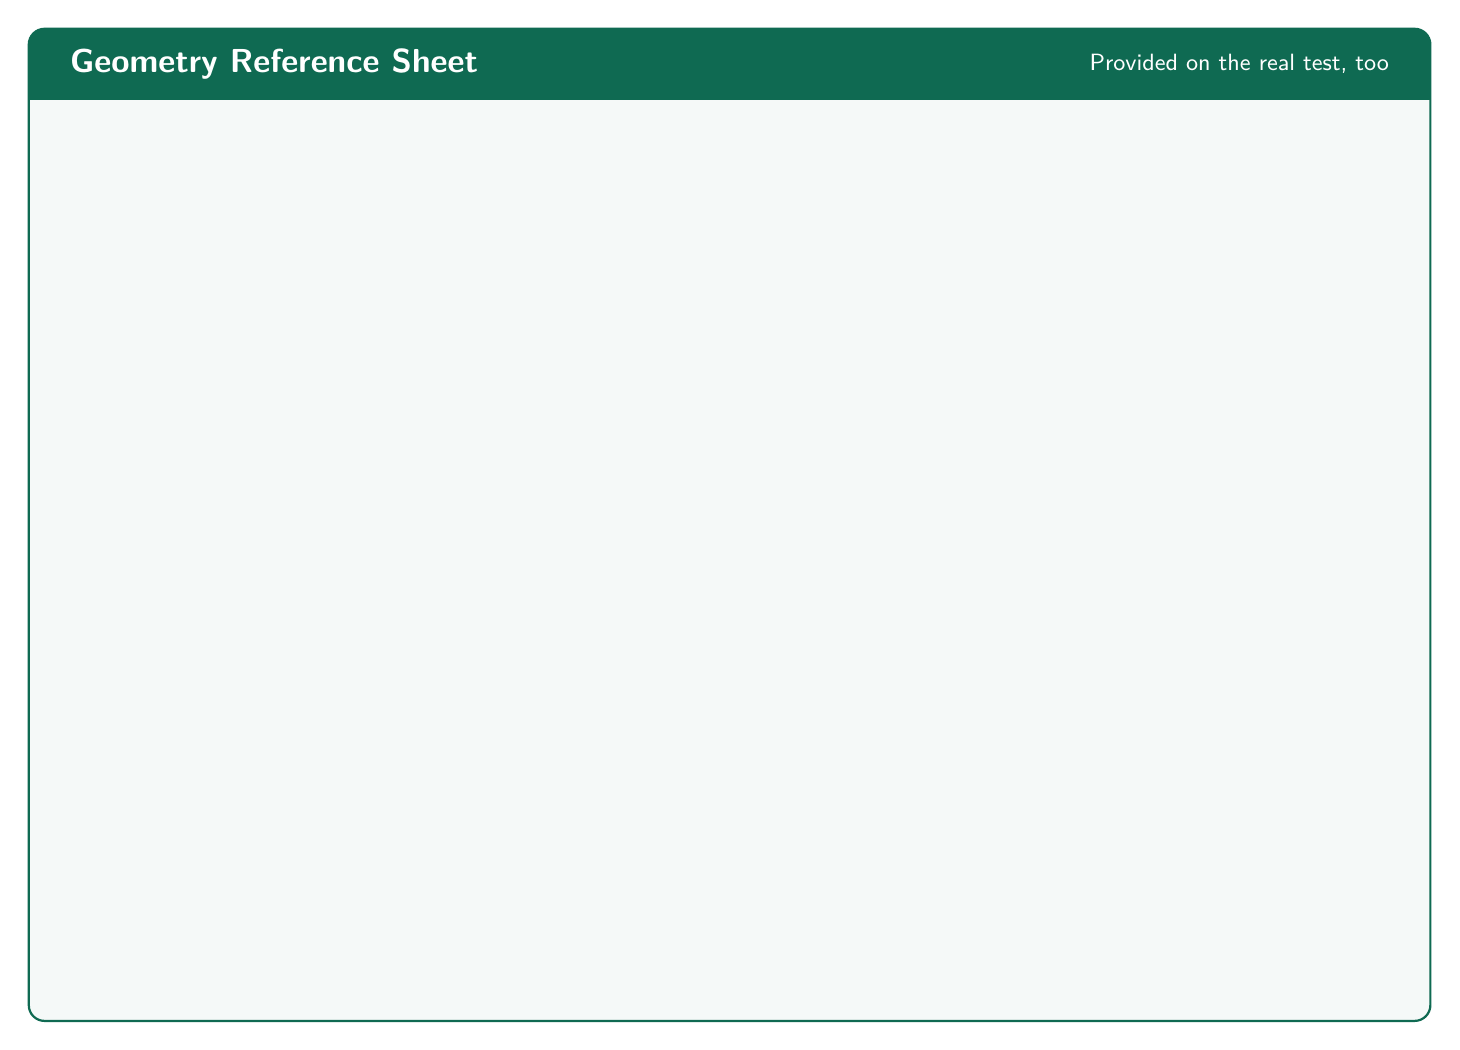
\begin{tikzpicture}
\draw[accent,line width=0.8pt,rounded corners=2mm,fill=badge!12] (0,0) rectangle (178mm,-126mm);
\fill[accent,rounded corners=2mm] (0,0) rectangle (178mm,-9mm);
\fill[accent] (0,-5mm) rectangle (178mm,-9mm);
\node[anchor=west,text=white,font=\sffamily\bfseries\fontsize{12}{14}\selectfont] at (4mm,-4.5mm) {Geometry Reference Sheet};
\node[anchor=east,text=white,font=\sffamily\fontsize{8.5}{10}\selectfont] at (174mm,-4.5mm) {Provided on the real test, too};
\end{tikzpicture}
\end{textblock*}

\newcommand{\refcell}[3]{\begin{textblock*}{42mm}(#1mm,#2mm)\begin{minipage}[t][36mm][t]{42mm}\centering #3\end{minipage}\end{textblock*}}
\newcommand{\refin}[2]{\parbox[b][26mm][b]{42mm}{\centering #1}\par\vspace{1.6mm}{\fontsize{9.6}{11.5}\selectfont #2}}
\tikzset{rf/.style={ink,line width=0.65pt},lb/.style={font=\fontsize{8.5}{9.5}\selectfont,inner sep=1.2pt}}

% ---------- row 1
\refcell{18}{167}{\refin{\begin{tikzpicture}[scale=1.25]
\draw[rf] (0,0) circle (9mm); \draw[rf] (0,0)--(9mm,0); \fill[ink] (0,0) circle (0.7pt);
\node[lb,above] at (4.5mm,0) {$r$};
\end{tikzpicture}}{Circle\\$A=\pi r^{2}$,\; $C=2\pi r$}}
\refcell{62}{167}{\refin{\begin{tikzpicture}[scale=1.25]
\draw[rf] (0,0) rectangle (22mm,12mm);
\node[lb,below] at (11mm,0) {$\ell$}; \node[lb,right] at (22mm,6mm) {$w$};
\end{tikzpicture}}{Rectangle\\$A=\ell w$}}
\refcell{106}{167}{\refin{\begin{tikzpicture}[scale=1.25]
\draw[rf] (0,0)--(22mm,0)--(7mm,13mm)--cycle;
\draw[rf,dashed] (7mm,0)--(7mm,13mm);
\draw[rf] (7mm,0)++(0,1.8mm)--++(1.8mm,0)--++(0,-1.8mm);
\node[lb,below] at (11mm,0) {$b$}; \node[lb,left] at (7mm,6.5mm) {$h$};
\end{tikzpicture}}{Triangle\\$A=\tfrac12 bh$}}
\refcell{150}{167}{\refin{\begin{tikzpicture}[scale=1.25]
\draw[rf] (0,0)--(18mm,0)--(0,12mm)--cycle;
\draw[rf] (0,1.8mm)--(1.8mm,1.8mm)--(1.8mm,0);
\node[lb,below] at (9mm,0) {$a$}; \node[lb,left] at (0,6mm) {$b$}; \node[lb,above right] at (9mm,6mm) {$c$};
\end{tikzpicture}}{Right triangle\\$c^{2}=a^{2}+b^{2}$}}

% ---------- row 2
\refcell{18}{204}{\refin{\begin{tikzpicture}[scale=1.25]
\draw[rf] (0,0)--(19.053mm,0)--(0,11mm)--cycle;
\draw[rf] (0,1.8mm)--(1.8mm,1.8mm)--(1.8mm,0);
\node[lb,below] at (9.5mm,0) {$x\sqrt3$}; \node[lb,left] at (0,5.5mm) {$x$}; \node[lb,above right] at (9.5mm,5.5mm) {$2x$};
\node[lb] at (14.6mm,1.9mm) {\fontsize{6.5}{7}\selectfont$30^\circ$}; \node[lb] at (3.2mm,8.2mm) {\fontsize{6.5}{7}\selectfont$60^\circ$};
\end{tikzpicture}}{$30^\circ$--$60^\circ$--$90^\circ$ triangle}}
\refcell{62}{204}{\refin{\begin{tikzpicture}[scale=1.25]
\draw[rf] (0,0)--(10mm,0)--(0,10mm)--cycle;
\draw[rf] (0,1.8mm)--(1.8mm,1.8mm)--(1.8mm,0);
\node[lb,below] at (5mm,0) {$s$}; \node[lb,left] at (0,5mm) {$s$}; \node[lb,above right] at (5mm,5mm) {$s\sqrt2$};
\end{tikzpicture}}{$45^\circ$--$45^\circ$--$90^\circ$ triangle}}
\refcell{106}{204}{\refin{\begin{tikzpicture}[scale=1.2]
\draw[rf] (0,0) rectangle (16mm,9mm);
\draw[rf] (16mm,9mm)--(22mm,13mm)--(6mm,13mm)--(0,9mm);
\draw[rf] (16mm,0)--(22mm,4mm)--(22mm,13mm);
\draw[rf,dashed] (6mm,13mm)--(6mm,4mm)--(22mm,4mm); \draw[rf,dashed] (0,0)--(6mm,4mm);
\node[lb,below] at (8mm,0) {$\ell$}; \node[lb,right] at (22mm,8.5mm) {$h$}; \node[lb,below right] at (19mm,2mm) {$w$};
\end{tikzpicture}}{Rectangular solid\\$V=\ell wh$}}
\refcell{150}{204}{\refin{\begin{tikzpicture}[scale=1.2]
\draw[rf] (0,2.2mm) ellipse (7mm and 2.2mm);
\draw[rf] (-7mm,2.2mm)--(-7mm,14mm); \draw[rf] (7mm,2.2mm)--(7mm,14mm);
\draw[rf] (0,14mm) ellipse (7mm and 2.2mm);
\draw[rf,dashed] (0,14mm)--(7mm,14mm); \fill[ink] (0,14mm) circle (0.6pt);
\node[lb,above] at (3.5mm,14mm) {$r$}; \node[lb,right] at (7mm,8mm) {$h$};
\end{tikzpicture}}{Right circular cylinder\\$V=\pi r^{2}h$}}

% ---------- row 3
\refcell{18}{241}{\refin{\begin{tikzpicture}[scale=1.15]
\draw[rf] (0,0) circle (10mm);
\draw[rf] (-10mm,0) arc (180:360:10mm and 2.8mm); \draw[rf,dashed] (-10mm,0) arc (180:0:10mm and 2.8mm);
\draw[rf] (0,0)--(10mm,0); \fill[ink] (0,0) circle (0.7pt); \node[lb,above] at (5mm,0) {$r$};
\end{tikzpicture}}{Sphere\\$V=\tfrac43\pi r^{3}$}}
\refcell{62}{241}{\refin{\begin{tikzpicture}[scale=1.2]
\draw[rf] (0,2.2mm) ellipse (7mm and 2.2mm);
\draw[rf] (-7mm,2.2mm)--(0,16mm)--(7mm,2.2mm);
\draw[rf,dashed] (0,16mm)--(0,2.2mm); \draw[rf,dashed] (0,2.2mm)--(7mm,2.2mm);
\fill[ink] (0,2.2mm) circle (0.6pt);
\node[lb,left] at (0,9.5mm) {$h$}; \node[lb,above] at (3.5mm,2.2mm) {$r$};
\end{tikzpicture}}{Right circular cone\\$V=\tfrac13\pi r^{2}h$}}
\refcell{106}{241}{\refin{\begin{tikzpicture}[scale=1.2]
\draw[rf] (0,0)--(16mm,0)--(22mm,4mm); \draw[rf] (0,0)--(10mm,15mm)--(16mm,0); \draw[rf] (10mm,15mm)--(22mm,4mm);
\draw[rf,dashed] (0,0)--(6mm,4mm)--(22mm,4mm); \draw[rf,dashed] (6mm,4mm)--(10mm,15mm);
\node[lb,below] at (8mm,0) {$\ell$}; \node[lb,below right] at (19mm,2mm) {$w$}; \node[lb,left] at (10mm,9.5mm) {$h$};
\end{tikzpicture}}{Rectangular pyramid\\$V=\tfrac13\ell wh$}}
\begin{textblock*}{40mm}(151mm,247mm)
{\fontsize{9.2}{12}\selectfont\raggedright
\textcolor{accent}{\rule[0.3mm]{1.6mm}{1.6mm}}\; A circle has 360 degrees of arc.\par\vspace{1.2mm}
\textcolor{accent}{\rule[0.3mm]{1.6mm}{1.6mm}}\; The angles of a triangle add up to 180 degrees.\par\vspace{1.2mm}
\textcolor{accent}{\rule[0.3mm]{1.6mm}{1.6mm}}\; $r$ radius, $\ell$ length, $w$ width, $b$ base, $h$ height.\par}
\end{textblock*}

\clearpage

% ===== Module 1, page 1 =====
\topicheader{6}{Mock Test 6}
\pagefooter{194}
\colrule{34}{236}
\mbox{}%
\pagekicker{Mock 6 \textperiodcentered{} Module 1 \textperiodcentered{} 22 questions \textperiodcentered{} 35 minutes}{Questions 1--8}
\begin{textblock*}{\COLW}(\LCOL,34mm)
{\fontsize{10.4}{13.4}\selectfont
\parbox[t][233mm][t]{\COLW}{%
\noindent\pnum{1} If $\dfrac{2}{3}x-5=7$, what is the value of $x$?\par\vspace{2.2mm}
\hspace*{7mm}(A)\ $8$\\[1.8mm]
\hspace*{7mm}(B)\ $13$\\[1.8mm]
\hspace*{7mm}(C)\ $18$\\[1.8mm]
\hspace*{7mm}(D)\ $36$
\vfill

\noindent\pnum{2} The graph of $y=(x-4)(x+2)$ in the $xy$-plane crosses the $x$-axis at two points. What is the distance between these two points?\par\vspace{2.2mm}
\hspace*{7mm}(A)\ $2$\\[1.8mm]
\hspace*{7mm}(B)\ $6$\\[1.8mm]
\hspace*{7mm}(C)\ $8$\\[1.8mm]
\hspace*{7mm}(D)\ $12$
\vfill

\noindent\pnum{3} A clinic has 1,600 patients enrolled. Exactly 45\% of them received a flu vaccination this season. How many of the enrolled patients did not receive a flu vaccination?\gridbox
\vfill

\noindent\pnum{4} In right triangle $ABC$, the right angle is at $C$, $AC=8$, and $BC=15$. What is the value of $\sin A$?\par\vspace{2.2mm}
\hspace*{7mm}(A)\ $\dfrac{8}{15}$\\[1.8mm]
\hspace*{7mm}(B)\ $\dfrac{8}{17}$\\[1.8mm]
\hspace*{7mm}(C)\ $\dfrac{15}{8}$\\[1.8mm]
\hspace*{7mm}(D)\ $\dfrac{15}{17}$
\vfill}}
\end{textblock*}
\begin{textblock*}{\COLW}(\RCOL,34mm)
{\fontsize{10.4}{13.4}\selectfont
\parbox[t][233mm][t]{\COLW}{%
\noindent\pnum{5} If $y=3x$ and $x+y=20$, what is the value of $x$?\par\vspace{2.2mm}
\hspace*{7mm}(A)\ $5$\\[1.8mm]
\hspace*{7mm}(B)\ $10$\\[1.8mm]
\hspace*{7mm}(C)\ $15$\\[1.8mm]
\hspace*{7mm}(D)\ $60$
\vfill

\noindent\pnum{6} Which of the following is equivalent to $4x^{2}-25$?\par\vspace{2.2mm}
\hspace*{7mm}(A)\ $(2x-5)(2x+5)$\\[1.8mm]
\hspace*{7mm}(B)\ $(2x-5)^{2}$\\[1.8mm]
\hspace*{7mm}(C)\ $(2x+5)^{2}$\\[1.8mm]
\hspace*{7mm}(D)\ $(4x-5)(x+5)$
\vfill

\noindent\pnum{7} The length of a rectangle is 4 inches more than twice its width. The perimeter of the rectangle is 44 inches. What is the width, in inches, of the rectangle?\gridbox
\vfill

\noindent\pnum{8} For $x>0$, which of the following is equivalent to $3x^{2}\cdot4x^{5}$?\par\vspace{2.2mm}
\hspace*{7mm}(A)\ $7x^{7}$\\[1.8mm]
\hspace*{7mm}(B)\ $7x^{10}$\\[1.8mm]
\hspace*{7mm}(C)\ $12x^{10}$\\[1.8mm]
\hspace*{7mm}(D)\ $12x^{7}$
\vfill}}
\end{textblock*}
\clearpage

% ===== Module 1, page 2 =====
\topicheader{6}{Mock Test 6}
\pagefooter{195}
\colrule{34}{236}
\mbox{}%
\pagekicker{Mock 6 \textperiodcentered{} Module 1 \textperiodcentered{} 22 questions \textperiodcentered{} 35 minutes}{Questions 9--15}
\begin{textblock*}{\COLW}(\LCOL,34mm)
{\fontsize{10.4}{13.4}\selectfont
\parbox[t][233mm][t]{\COLW}{%
\noindent\pnum{9} The scatterplot shows data for 12 basketball players. For each player, $x$ is the average number of minutes played per game and $y$ is the average number of points scored per game. The line of best fit shown has equation $y=0.62x-3.4$. Which of the following is the best interpretation of the number 0.62 in this context?\figwrap{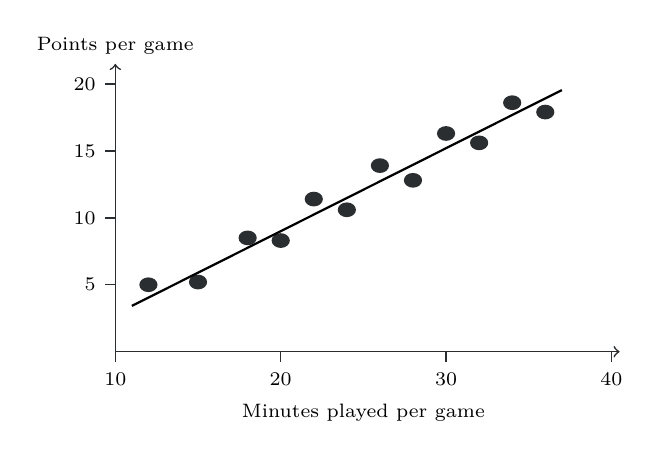
\begin{tikzpicture}[x=2.1mm,y=1.7mm]
\draw[->,ink,line width=0.6pt] (10,0)--(40.5,0);
\draw[->,ink,line width=0.6pt] (10,0)--(10,21.5);
\foreach \a in {10,20,30,40}{\draw[ink,line width=0.5pt] (\a,0)--(\a,-0.8); \node[below,font=\scriptsize] at (\a,-0.8) {\a};}
\foreach \b in {5,10,15,20}{\draw[ink,line width=0.5pt] (10,\b)--(9.4,\b); \node[left,font=\scriptsize] at (9.4,\b) {\b};}
\node[below,font=\scriptsize] at (25,-3.2) {Minutes played per game};
\node[above,font=\scriptsize] at (10,21.5) {Points per game};
\foreach \a/\b in {12/5.0,15/5.2,18/8.5,20/8.3,22/11.4,24/10.6,26/13.9,28/12.8,30/16.3,32/15.6,34/18.6,36/17.9}{\fill[ink] (\a,\b) circle (0.55);}
\draw[line width=0.8pt] (11,3.42)--(37,19.54);
\end{tikzpicture}}\par\vspace{2.2mm}
\hspace*{7mm}(A)\ A player who plays 0 minutes per game is predicted to score 0.62 points per game.\\[1.8mm]
\hspace*{7mm}(B)\ The players in the data set scored 0.62 points per game on average.\\[1.8mm]
\hspace*{7mm}(C)\ For each additional minute played per game, the predicted number of points scored per game increases by 0.62.\\[1.8mm]
\hspace*{7mm}(D)\ For each additional point scored per game, the predicted number of minutes played per game increases by 0.62.
\vfill

\noindent\pnum{10} A homebuyer makes a down payment of \$24,000 and then pays \$1,350 each month. What is the least whole number of months after which the total amount paid, including the down payment, will exceed \$90,000?\par\vspace{2.2mm}
\hspace*{7mm}(A)\ $48$\\[1.8mm]
\hspace*{7mm}(B)\ $49$\\[1.8mm]
\hspace*{7mm}(C)\ $66$\\[1.8mm]
\hspace*{7mm}(D)\ $67$
\vfill

\noindent\pnum{11} The lines $3x+2y=16$ and $x-y=2$ intersect at a point in the $xy$-plane. The line $y=kx+10$, where $k$ is a constant, passes through the same point. What is the value of $k$?\gridbox
\vfill}}
\end{textblock*}
\begin{textblock*}{\COLW}(\RCOL,34mm)
{\fontsize{10.4}{13.4}\selectfont
\parbox[t][233mm][t]{\COLW}{%
\noindent\pnum{12} The phosphate level in a lake is 50 units today and decreases by 12\% every 3 years. Which of the following functions gives the phosphate level $P(t)$, in units, $t$ years from today?\par\vspace{2.2mm}
\hspace*{7mm}(A)\ $P(t)=50(0.88)^{t/3}$\\[1.8mm]
\hspace*{7mm}(B)\ $P(t)=50(0.88)^{3t}$\\[1.8mm]
\hspace*{7mm}(C)\ $P(t)=50(0.12)^{t/3}$\\[1.8mm]
\hspace*{7mm}(D)\ $P(t)=50(1.12)^{t/3}$
\vfill

\noindent\pnum{13} A surveyor whose eyes are 1.6 meters above the ground stands on level ground 50 meters from the base of a tower. The angle of elevation from the surveyor's eyes to the top of the tower is $55^{\circ}$. To the nearest meter, what is the height of the tower?\par\vspace{2.2mm}
\hspace*{7mm}(A)\ $35$\\[1.8mm]
\hspace*{7mm}(B)\ $41$\\[1.8mm]
\hspace*{7mm}(C)\ $71$\\[1.8mm]
\hspace*{7mm}(D)\ $73$
\vfill

\noindent\pnum{14} The functions $f$ and $g$ are defined by $f(x)=3x-2$ and $g(x)=x^{2}+1$. If $x>0$ and $f(g(x))=49$, what is the value of $x$?\gridbox
\vfill

\noindent\pnum{15} A fiber-optic line transfers data at 480 megabits per second. At this rate, how many gigabytes of data can the line transfer in 10 minutes? (1 byte $=8$ bits and 1 gigabyte $=1{,}000$ megabytes.)\par\vspace{2.2mm}
\hspace*{7mm}(A)\ $0.6$\\[1.8mm]
\hspace*{7mm}(B)\ $3.6$\\[1.8mm]
\hspace*{7mm}(C)\ $36$\\[1.8mm]
\hspace*{7mm}(D)\ $288$
\vfill}}
\end{textblock*}
\clearpage

% ===== Module 1, page 3 =====
\topicheader{6}{Mock Test 6}
\pagefooter{196}
\colrule{34}{236}
\mbox{}%
\pagekicker{Mock 6 \textperiodcentered{} Module 1 \textperiodcentered{} 22 questions \textperiodcentered{} 35 minutes}{Questions 16--22}
\begin{textblock*}{\COLW}(\LCOL,34mm)
{\fontsize{10.4}{13.4}\selectfont
\parbox[t][233mm][t]{\COLW}{%
\noindent\pnum{16} A food truck sells tacos for \$3 each and burritos for \$7.50 each. On days when its revenue is exactly \$600, the numbers of tacos $t$ and burritos $b$ sold satisfy $3t+7.5b=600$. According to this equation, each additional burrito sold corresponds to how many fewer tacos sold?\par\vspace{2.2mm}
\hspace*{7mm}(A)\ $0.4$\\[1.8mm]
\hspace*{7mm}(B)\ $2.5$\\[1.8mm]
\hspace*{7mm}(C)\ $4.5$\\[1.8mm]
\hspace*{7mm}(D)\ $7.5$
\vfill

\noindent\pnum{17} The graphs of $y=x^{2}-3x-4$ and $y=2x+2$ in the $xy$-plane intersect at two points. What is the $y$-coordinate of the point of intersection with the greater $x$-coordinate?\par\vspace{2.2mm}
\hspace*{7mm}(A)\ $0$\\[1.8mm]
\hspace*{7mm}(B)\ $2$\\[1.8mm]
\hspace*{7mm}(C)\ $6$\\[1.8mm]
\hspace*{7mm}(D)\ $14$
\vfill

\noindent\pnum{18} If $x>0$, $y>0$, $x^{2}+y^{2}=52$, and $xy=24$, what is the value of $x+y$?\gridbox
\vfill

\noindent\pnum{19} In the $xy$-plane, line $\ell$ passes through the points $(2,-3)$ and $(8,9)$. Line $m$ is perpendicular to $\ell$ and passes through the origin. Which of the following points lies on line $m$?\par\vspace{2.2mm}
\hspace*{7mm}(A)\ $(4,-2)$\\[1.8mm]
\hspace*{7mm}(B)\ $(2,-4)$\\[1.8mm]
\hspace*{7mm}(C)\ $(4,2)$\\[1.8mm]
\hspace*{7mm}(D)\ $(2,4)$
\vfill}}
\end{textblock*}
\begin{textblock*}{\COLW}(\RCOL,34mm)
{\fontsize{10.4}{13.4}\selectfont
\parbox[t][233mm][t]{\COLW}{%
\noindent\pnum{20} In the $xy$-plane, the line $3x+4y=36$ crosses the $x$-axis at point $A$ and the $y$-axis at point $B$. What is the shortest distance, in units, from the origin to line segment $\overline{AB}$?\par\vspace{2.2mm}
\hspace*{7mm}(A)\ $\dfrac{36}{7}$\\[1.8mm]
\hspace*{7mm}(B)\ $\dfrac{36}{5}$\\[1.8mm]
\hspace*{7mm}(C)\ $\dfrac{15}{2}$\\[1.8mm]
\hspace*{7mm}(D)\ $9$
\vfill

\noindent\pnum{21} In the equation $x^{2}-kx+18=0$, $k$ is a positive constant. The two solutions of the equation differ by 3. What is the value of $k$?\gridbox
\vfill

\noindent\pnum{22} Print Shop A charges \$0.50 per page for the first 200 pages of an order and \$0.30 for each page after the first 200. Print Shop B charges a flat \$60 plus \$0.10 per page. What is the least number of pages for which Print Shop B's total charge is strictly less than Print Shop A's?\par\vspace{2.2mm}
\hspace*{7mm}(A)\ $101$\\[1.8mm]
\hspace*{7mm}(B)\ $150$\\[1.8mm]
\hspace*{7mm}(C)\ $151$\\[1.8mm]
\hspace*{7mm}(D)\ $200$
\vfill}}
\end{textblock*}
\clearpage

% ===== Module 2, page 1 =====
\topicheader{6}{Mock Test 6}
\pagefooter{197}
\colrule{34}{236}
\mbox{}%
\pagekicker{Mock 6 \textperiodcentered{} Module 2 \textperiodcentered{} 22 questions \textperiodcentered{} 35 minutes}{Questions 1--8}
\begin{textblock*}{\COLW}(\LCOL,34mm)
{\fontsize{10.4}{13.4}\selectfont
\parbox[t][233mm][t]{\COLW}{%
\noindent\pnum{1} If $5(x-3)=2x+9$, what is the value of $x$?\par\vspace{2.2mm}
\hspace*{7mm}(A)\ $-2$\\[1.8mm]
\hspace*{7mm}(B)\ $2$\\[1.8mm]
\hspace*{7mm}(C)\ $4$\\[1.8mm]
\hspace*{7mm}(D)\ $8$
\vfill

\noindent\pnum{2} What is the $x$-coordinate of the vertex of the graph of $y=x^{2}-6x+11$ in the $xy$-plane?\par\vspace{2.2mm}
\hspace*{7mm}(A)\ $-3$\\[1.8mm]
\hspace*{7mm}(B)\ $3$\\[1.8mm]
\hspace*{7mm}(C)\ $6$\\[1.8mm]
\hspace*{7mm}(D)\ $11$
\vfill

\noindent\pnum{3} The body mass index $B$ of a person who weighs $w$ pounds and is $h$ inches tall is given by $B=\dfrac{703w}{h^{2}}$. Which of the following expresses $h$ in terms of $B$ and $w$, for $h>0$?\par\vspace{2.2mm}
\hspace*{7mm}(A)\ $h=\dfrac{\sqrt{703w}}{B}$\\[1.8mm]
\hspace*{7mm}(B)\ $h=\left(\dfrac{703w}{B}\right)^{2}$\\[1.8mm]
\hspace*{7mm}(C)\ $h=\dfrac{703w}{\sqrt{B}}$\\[1.8mm]
\hspace*{7mm}(D)\ $h=\sqrt{\dfrac{703w}{B}}$
\vfill

\noindent\pnum{4} A no-interest loan is repaid in equal monthly payments, so the remaining balance decreases by the same amount each month. After 8 months the remaining balance is \$9,360, and after 20 months it is \$7,200. What was the original loan amount, in dollars?\gridbox
\vfill}}
\end{textblock*}
\begin{textblock*}{\COLW}(\RCOL,34mm)
{\fontsize{10.4}{13.4}\selectfont
\parbox[t][233mm][t]{\COLW}{%
\noindent\pnum{5} The number of reported cases of a virus in a town grew exponentially, with 250 cases in week 0 and 360 cases in week 2. By what percent did the number of reported cases grow each week?\par\vspace{2.2mm}
\hspace*{7mm}(A)\ $20\%$\\[1.8mm]
\hspace*{7mm}(B)\ $22\%$\\[1.8mm]
\hspace*{7mm}(C)\ $44\%$\\[1.8mm]
\hspace*{7mm}(D)\ $120\%$
\vfill

\noindent\pnum{6} Two triangular sails are similar. The smaller sail has an area of 18 square feet, and the larger sail has an area of 72 square feet. A side of the smaller sail is 5 feet long. How long, in feet, is the corresponding side of the larger sail?\par\vspace{2.2mm}
\hspace*{7mm}(A)\ $10$\\[1.8mm]
\hspace*{7mm}(B)\ $20$\\[1.8mm]
\hspace*{7mm}(C)\ $54$\\[1.8mm]
\hspace*{7mm}(D)\ $90$
\vfill

\noindent\pnum{7} The graph of $y=|3x-12|-6$ and the line $y=9$ intersect at two points in the $xy$-plane. What is the distance between these two points?\par\vspace{2.2mm}
\hspace*{7mm}(A)\ $2$\\[1.8mm]
\hspace*{7mm}(B)\ $9$\\[1.8mm]
\hspace*{7mm}(C)\ $10$\\[1.8mm]
\hspace*{7mm}(D)\ $30$
\vfill

\noindent\pnum{8} What is the sum of the squares of the three real solutions of the equation $x^{3}-5x^{2}-4x+20=0$?\gridbox
\vfill}}
\end{textblock*}
\clearpage

% ===== Module 2, page 2 =====
\topicheader{6}{Mock Test 6}
\pagefooter{198}
\colrule{34}{236}
\mbox{}%
\pagekicker{Mock 6 \textperiodcentered{} Module 2 \textperiodcentered{} 22 questions \textperiodcentered{} 35 minutes}{Questions 9--15}
\begin{textblock*}{\COLW}(\LCOL,34mm)
{\fontsize{10.4}{13.4}\selectfont
\parbox[t][233mm][t]{\COLW}{%
\noindent\pnum{9} Which of the following quadratic equations has the solutions $x=3+\sqrt{7}$ and $x=3-\sqrt{7}$?\par\vspace{2.2mm}
\hspace*{7mm}(A)\ $x^{2}-6x+2=0$\\[1.8mm]
\hspace*{7mm}(B)\ $x^{2}-6x-2=0$\\[1.8mm]
\hspace*{7mm}(C)\ $x^{2}+6x+2=0$\\[1.8mm]
\hspace*{7mm}(D)\ $x^{2}-6x+16=0$
\vfill

\noindent\pnum{10} Glacier A is 420 meters thick and is thinning at a constant rate of 3.5 meters per decade. Glacier B is 350 meters thick and is thinning at a constant rate of 1.5 meters per decade. What is the least whole number of decades after which Glacier A will be thinner than Glacier B?\par\vspace{2.2mm}
\hspace*{7mm}(A)\ $35$\\[1.8mm]
\hspace*{7mm}(B)\ $36$\\[1.8mm]
\hspace*{7mm}(C)\ $70$\\[1.8mm]
\hspace*{7mm}(D)\ $120$
\vfill

\noindent\pnum{11} A mobile plan costs \$45 per month and includes 10 gigabytes (GB) of data. Each additional whole gigabyte used costs \$8.50. Jin wants her bill for a month to be at most \$120. What is the greatest whole number of gigabytes in total that she can use in that month?\gridbox
\vfill

\noindent\pnum{12} If $\dfrac{x}{2}+\dfrac{y}{3}=7$ and $\dfrac{x}{4}-\dfrac{y}{6}=\dfrac{3}{2}$, what is the value of $xy$?\par\vspace{2.2mm}
\hspace*{7mm}(A)\ $4$\\[1.8mm]
\hspace*{7mm}(B)\ $16$\\[1.8mm]
\hspace*{7mm}(C)\ $60$\\[1.8mm]
\hspace*{7mm}(D)\ $120$
\vfill}}
\end{textblock*}
\begin{textblock*}{\COLW}(\RCOL,34mm)
{\fontsize{10.4}{13.4}\selectfont
\parbox[t][233mm][t]{\COLW}{%
\noindent\pnum{13} Researchers wanted to know whether a new walking program lowers blood pressure in patients aged 50 to 65 at a health system. They selected 400 such patients at random and invited them to join; each patient decided whether to join. After six months, the average drop in systolic blood pressure was 9 points for the 210 patients who joined and 3 points for the 190 who did not. Which conclusion is best supported by the study?\par\vspace{2.2mm}
\hspace*{7mm}(A)\ The program causes a larger drop in blood pressure for all patients aged 50 to 65 at the health system.\\[1.8mm]
\hspace*{7mm}(B)\ The program causes a larger drop in blood pressure for the 400 patients selected, but this cannot be generalized to other patients.\\[1.8mm]
\hspace*{7mm}(C)\ Because patients chose whether to join, nothing can be concluded about patients other than the 400 selected.\\[1.8mm]
\hspace*{7mm}(D)\ Among patients aged 50 to 65 at the health system, joining is associated with a larger drop in blood pressure, but the study does not show that the program caused the larger drop.
\vfill

\noindent\pnum{14} The concentration of a herbicide in a pond, in micrograms per liter, $d$ days after it was applied is modeled by $C(d)=64(0.8)^{d/5}$. According to the model, the concentration decreases by 36\% every $n$ days. What is the value of $n$?\par\vspace{2.2mm}
\hspace*{7mm}(A)\ $5$\\[1.8mm]
\hspace*{7mm}(B)\ $10$\\[1.8mm]
\hspace*{7mm}(C)\ $25$\\[1.8mm]
\hspace*{7mm}(D)\ $36$
\vfill

\noindent\pnum{15} A city planner surveyed two independent random samples of residents about a proposed bike lane. In the first sample, 38\% of the respondents supported the proposal, with a margin of error of 3.1 percentage points. In the second sample, 43\% supported it, with a margin of error of 3.4 percentage points. Both margins of error were calculated at the same confidence level. Which of the following percentages of all residents who support the proposal is consistent with the results of both samples?\par\vspace{2.2mm}
\hspace*{7mm}(A)\ $36\%$\\[1.8mm]
\hspace*{7mm}(B)\ $38\%$\\[1.8mm]
\hspace*{7mm}(C)\ $40\%$\\[1.8mm]
\hspace*{7mm}(D)\ $43\%$
\vfill}}
\end{textblock*}
\clearpage

% ===== Module 2, page 3 =====
\topicheader{6}{Mock Test 6}
\pagefooter{199}
\colrule{34}{236}
\mbox{}%
\pagekicker{Mock 6 \textperiodcentered{} Module 2 \textperiodcentered{} 22 questions \textperiodcentered{} 35 minutes}{Questions 16--22}
\begin{textblock*}{\COLW}(\LCOL,34mm)
{\fontsize{10.4}{13.4}\selectfont
\parbox[t][233mm][t]{\COLW}{%
\noindent\pnum{16} In the $xy$-plane, the graph of the equation below is a circle.\dsp{$x^{2}+y^{2}-12x-16y+84=0$}What is the shortest distance, in units, from the origin to a point on the circle?\gridbox
\vfill

\noindent\pnum{17} A runner jogs the first half of a trail's length at 6 miles per hour and the second half at a constant speed of $v$ miles per hour. Her average speed for the entire trail is 8 miles per hour. What is the value of $v$?\par\vspace{2.2mm}
\hspace*{7mm}(A)\ $10$\\[1.8mm]
\hspace*{7mm}(B)\ $12$\\[1.8mm]
\hspace*{7mm}(C)\ $14$\\[1.8mm]
\hspace*{7mm}(D)\ $16$
\vfill

\noindent\pnum{18} A screening test for a virus is given to everyone in a large population. The table shows the percent of the population in each group and the percent of each group that tests positive. Of all the people who test positive, approximately what percent are actually infected?\figwrap{\begin{tabular}{|l|>{\centering\arraybackslash}p{22mm}|>{\centering\arraybackslash}p{27mm}|}
\hline
Group & Share of the population & Percent who test positive\\\hline
Infected & 2\% & 90\%\\\hline
Not infected & 98\% & 5\%\\\hline
\end{tabular}}\par\vspace{2.2mm}
\hspace*{7mm}(A)\ $2\%$\\[1.8mm]
\hspace*{7mm}(B)\ $27\%$\\[1.8mm]
\hspace*{7mm}(C)\ $90\%$\\[1.8mm]
\hspace*{7mm}(D)\ $95\%$
\vfill}}
\end{textblock*}
\begin{textblock*}{\COLW}(\RCOL,34mm)
{\fontsize{10.4}{13.4}\selectfont
\parbox[t][233mm][t]{\COLW}{%
\noindent\pnum{19} For a positive constant $k$, how many distinct real solutions does the equation $x^{2}-8x+16=k\,|x-4|$ have?\par\vspace{2.2mm}
\hspace*{7mm}(A)\ $1$\\[1.8mm]
\hspace*{7mm}(B)\ $2$\\[1.8mm]
\hspace*{7mm}(C)\ $3$\\[1.8mm]
\hspace*{7mm}(D)\ $4$
\vfill

\noindent\pnum{20} For a constant $k$, the vertex of the parabola $y=x^{2}-4kx+3k$ lies on the line $y=2x-5$. What is the sum of all possible values of $k$?\gridbox
\vfill

\noindent\pnum{21} What is the sum of all real solutions of the equation $|x-2|+|x-9|=15$?\par\vspace{2.2mm}
\hspace*{7mm}(A)\ $11$\\[1.8mm]
\hspace*{7mm}(B)\ $13$\\[1.8mm]
\hspace*{7mm}(C)\ $15$\\[1.8mm]
\hspace*{7mm}(D)\ $22$
\vfill

\noindent\pnum{22} From a point on level ground, the angle of elevation to the top of a wind turbine's tower is $28^{\circ}$. After walking 40 meters directly toward the base of the tower, the observer measures the angle of elevation to the top as $41^{\circ}$. Ignoring the observer's height, to the nearest meter, how tall is the tower?\par\vspace{2.2mm}
\hspace*{7mm}(A)\ $9$\\[1.8mm]
\hspace*{7mm}(B)\ $21$\\[1.8mm]
\hspace*{7mm}(C)\ $35$\\[1.8mm]
\hspace*{7mm}(D)\ $55$
\vfill}}
\end{textblock*}
\clearpage

\end{document}
